%% Postdoctoral Research Statement
%% Adapted from the SOP template at
%% http://tex.stackexchange.com/questions/150900/latex-coding-for-statement-of-purpose
%%
%% Compile with:  pdflatex -> bibtex -> pdflatex -> pdflatex
%% Requires references.bib alongside this file.

\documentclass[11pt]{article}
\usepackage[
  a4paper,
  margin=1in,
  headsep=3pt, % separation between header rule and text
]{geometry}
\usepackage{xcolor}
\usepackage{fancyhdr}
\usepackage{scholax}
\usepackage{lastpage}
\usepackage{enumitem}
\usepackage{wrapfig}
\usepackage{graphicx}
\usepackage{subcaption}
\usepackage{xcolor}
\usepackage{marginnote}
\usepackage{caption}
\DeclareCaptionFont{customsizefig}{\fontsize{10pt}{10pt}\selectfont}
\DeclareCaptionFont{customsizesubfig}{\fontsize{9pt}{9pt}\selectfont}
\captionsetup[figure]{font=customsizefig}
\captionsetup[subfigure]{font=customsizesubfig}
\newcommand{\TODO}[1]{%
  \marginnote{\color{red}\textbf{TODO}}% Put 'TODO' in margin
  {\color{red}#1}% Put the associated text in red in the body
}

%% ---------------------------------------------------------------
%% Bibliography: natbib + BibTeX, author-year style.  Cite in-line
%% with \citep{key} (parenthetical) or \citet{key} (textual).
%% ---------------------------------------------------------------
\usepackage[round,authoryear]{natbib}
\bibliographystyle{ieeetr}
\setlength{\bibsep}{2pt plus 0.3ex}

\pagestyle{fancy}
\fancyhf{}
\fancyhead[C]{%
  \footnotesize\sffamily
  web: \textcolor{blue}{\yourweb}\quad
  \yourname\quad
  email: \textcolor{blue}{\youremail}}
\fancyfoot[C]{Page \thepage\ of \pageref{LastPage}}

%% ---------------------------------------------------------------
%% Personal-info macros: edit these once, they propagate everywhere.
%% ---------------------------------------------------------------
\newcommand{\yourname}{Sean Patrick MacBride}
\newcommand{\youremail}{\href{mailto:sean.macbride@physik.uzh.ch}{sean.macbride@physik.uzh.ch}}
\newcommand{\yourweb}{\href{https://seanmacb.github.io}{seanmacb.github.io}}

\newcommand{\hindex}{8}
\newcommand{\hindexDate}{August 2026}

\newcommand{\soptitle}{Research Statement}

%% Section-header macro (kept from the original SOP template)
\newcommand{\statement}[1]{\par\medskip
  \textcolor{blue}{\textbf{#1:}}%\hspace{0.05cm}
}

%% Highlight macro for spots the author should tailor per application
%% (e.g. naming the specific host group, fellowship, or institution).
\newcommand{\fillin}[1]{\textcolor{orange}{\textbf{[#1]}}}

%% ---------------------------------------------------------------
%% Recurring survey / collaboration / instrument acronyms.
%%
%% These are now managed by the `acro' package: each is declared once
%% with a long and a short form, and \ac{...} automatically prints
%% "Long Form (SHORT)" on first use and "SHORT" every time after.
%% The user-facing macros (\LSST, \DESC, ...) are kept unchanged so
%% the body text below did not have to be rewritten.
%% ---------------------------------------------------------------
\usepackage{acro}
\acsetup{make-links=false}

\DeclareAcronym{lsst}    {short = LSST,    long = Legacy Survey of Space and Time}
\DeclareAcronym{lsstcam} {short = LSSTCam, long = LSST Camera}
\DeclareAcronym{desc}    {short = DESC,    long = LSST-Dark Energy Science Collaboration}
\DeclareAcronym{des}     {short = DES,     long = Dark Energy Survey}
\DeclareAcronym{desi}    {short = DESI,    long = Dark Energy Spectroscopic Instrument}
\DeclareAcronym{desgw}   {short = DESGW,   long = Dark Energy Survey Gravitational Wave follow-up program}
\DeclareAcronym{delve}   {short = DELVE,   long = Dark Energy Local Volume Exploration}
\DeclareAcronym{pfs}     {short = PFS,     long = Prime Focus Spectrograph}
\DeclareAcronym{llamas}  {short = LLAMAS,  long = Large Lenslet Array Magellan Spectrograph}
\DeclareAcronym{igwn}    {short = IGWN,    long = International Gravitational Wave Network}
\DeclareAcronym{lvk}     {short = LVK,     long = LIGO-Virgo-Kagra}
\DeclareAcronym{too}     {short = ToO,     long = Target-of-Opportunity}
\DeclareAcronym{decam}   {short = DECam,   long = Dark Energy Camera}
\DeclareAcronym{rubin}   {short = Rubin,   long = Vera C. Rubin Observatory}
\DeclareAcronym{must}   {short = MUST,   long = MUltiplexed Survey Telescope}
\DeclareAcronym{3G}   {short = 3G,   long = third generation}

\DeclareAcronym{specsfive}   {short = Spec-S5,   long = Stage-5 Spectroscopic Experiment}
\DeclareAcronym{LISA}   {short = LISA,   long = Laser Interferometer Space Antenna}
\DeclareAcronym{hyperk}   {short = Hyper-K,   long = Hyper Kamiokande}
\DeclareAcronym{DUNE}   {short = DUNE,   long = Deep Underground Neutrino Experiment}
\DeclareAcronym{jgem}    {short = J-GEM,
                          long  = Japanese collaboration for gravitational-wave electromagnetic follow-up}
\DeclareAcronym{UNIONS}   {short = UNIONS,   long = The Ultraviolet Near-infrared Optical Northern Survey} 

\newcommand{\LSST}{\ac{lsst}}
\newcommand{\threeG}{\ac{3G}}
\newcommand{\UNIONS}{\ac{UNIONS}}
\newcommand{\LSSTCam}{\ac{lsstcam}}
\newcommand{\DESC}{\ac{desc}}
\newcommand{\DES}{\ac{des}}
\newcommand{\DESI}{\ac{desi}}
\newcommand{\DESGW}{\ac{desgw}}
\newcommand{\DELVE}{\ac{delve}}
\newcommand{\PFS}{\ac{pfs}}
\newcommand{\LLAMAS}{\ac{llamas}}
\newcommand{\IGWN}{\ac{igwn}}
\newcommand{\LVK}{\ac{lvk}}
\newcommand{\ToO}{\ac{too}}
\newcommand{\DECam}{\ac{decam}}
\newcommand{\JGEM}{\ac{jgem}}
\newcommand{\must}{\ac{must}}

\newcommand{\specsfive}{\ac{specsfive}}
\newcommand{\LISA}{\ac{LISA}}
\newcommand{\hyperk}{\ac{hyperk}}
\newcommand{\DUNE}{\ac{DUNE}}

%% Non-acronym text macros (unchanged: these are names, not abbreviations)
\newcommand{\Rubin}{\ac{rubin}}
\newcommand{\Ho}{\ensuremath{H_0}}
\newcommand{\Blanco}{V\'ictor M. Blanco 4-meter Telescope}
\newcommand{\IceCube}{IceCube Neutrino Observatory}
\newcommand{\Institute}{\TODO{Add Institution}}

\usepackage[
  breaklinks,
  pdftitle={\yourname - \soptitle},
  pdfauthor={\yourname},
  unicode
]{hyperref}

\begin{document}
\begin{center}\vspace{2pt}\LARGE\soptitle\\
\large \yourname\\
\vspace{2pt}
\end{center}
\hrule
\vspace{2pt}
\hrule height 1pt
\bigskip
My research focuses on exploring the cosmic frontier using electromagnetic and gravitational wave data.
This focus is underscored by three distinct pillars: building cutting-edge astronomical instrumentation, leading observing campaigns to search for the electromagnetic counterparts to gravitational-wave mergers, and performing inference on electromagnetic and gravitational-wave data to achieve robust cosmological constraints.
These three pillars reflect the approach I aim to bring to \Institute, where each research activity is not viewed as separate, but as three legs of one research program, strongest when pursued together. 
\begin{figure*}[bh]
    \centering
    \begin{subfigure}[b]{0.32\textwidth}
        \centering
        \includegraphics[width=\textwidth]{figures/placeholder.pdf}
        \caption{Removal of the persistence effect, a dominant residual charge effect in LSSTCam sensors \cite{MacBride2026LSSTCam}.}
        \label{fig:highlights:lsstcam}
    \end{subfigure}%
    \hfill
    \begin{subfigure}[b]{0.32\textwidth}
        \centering
        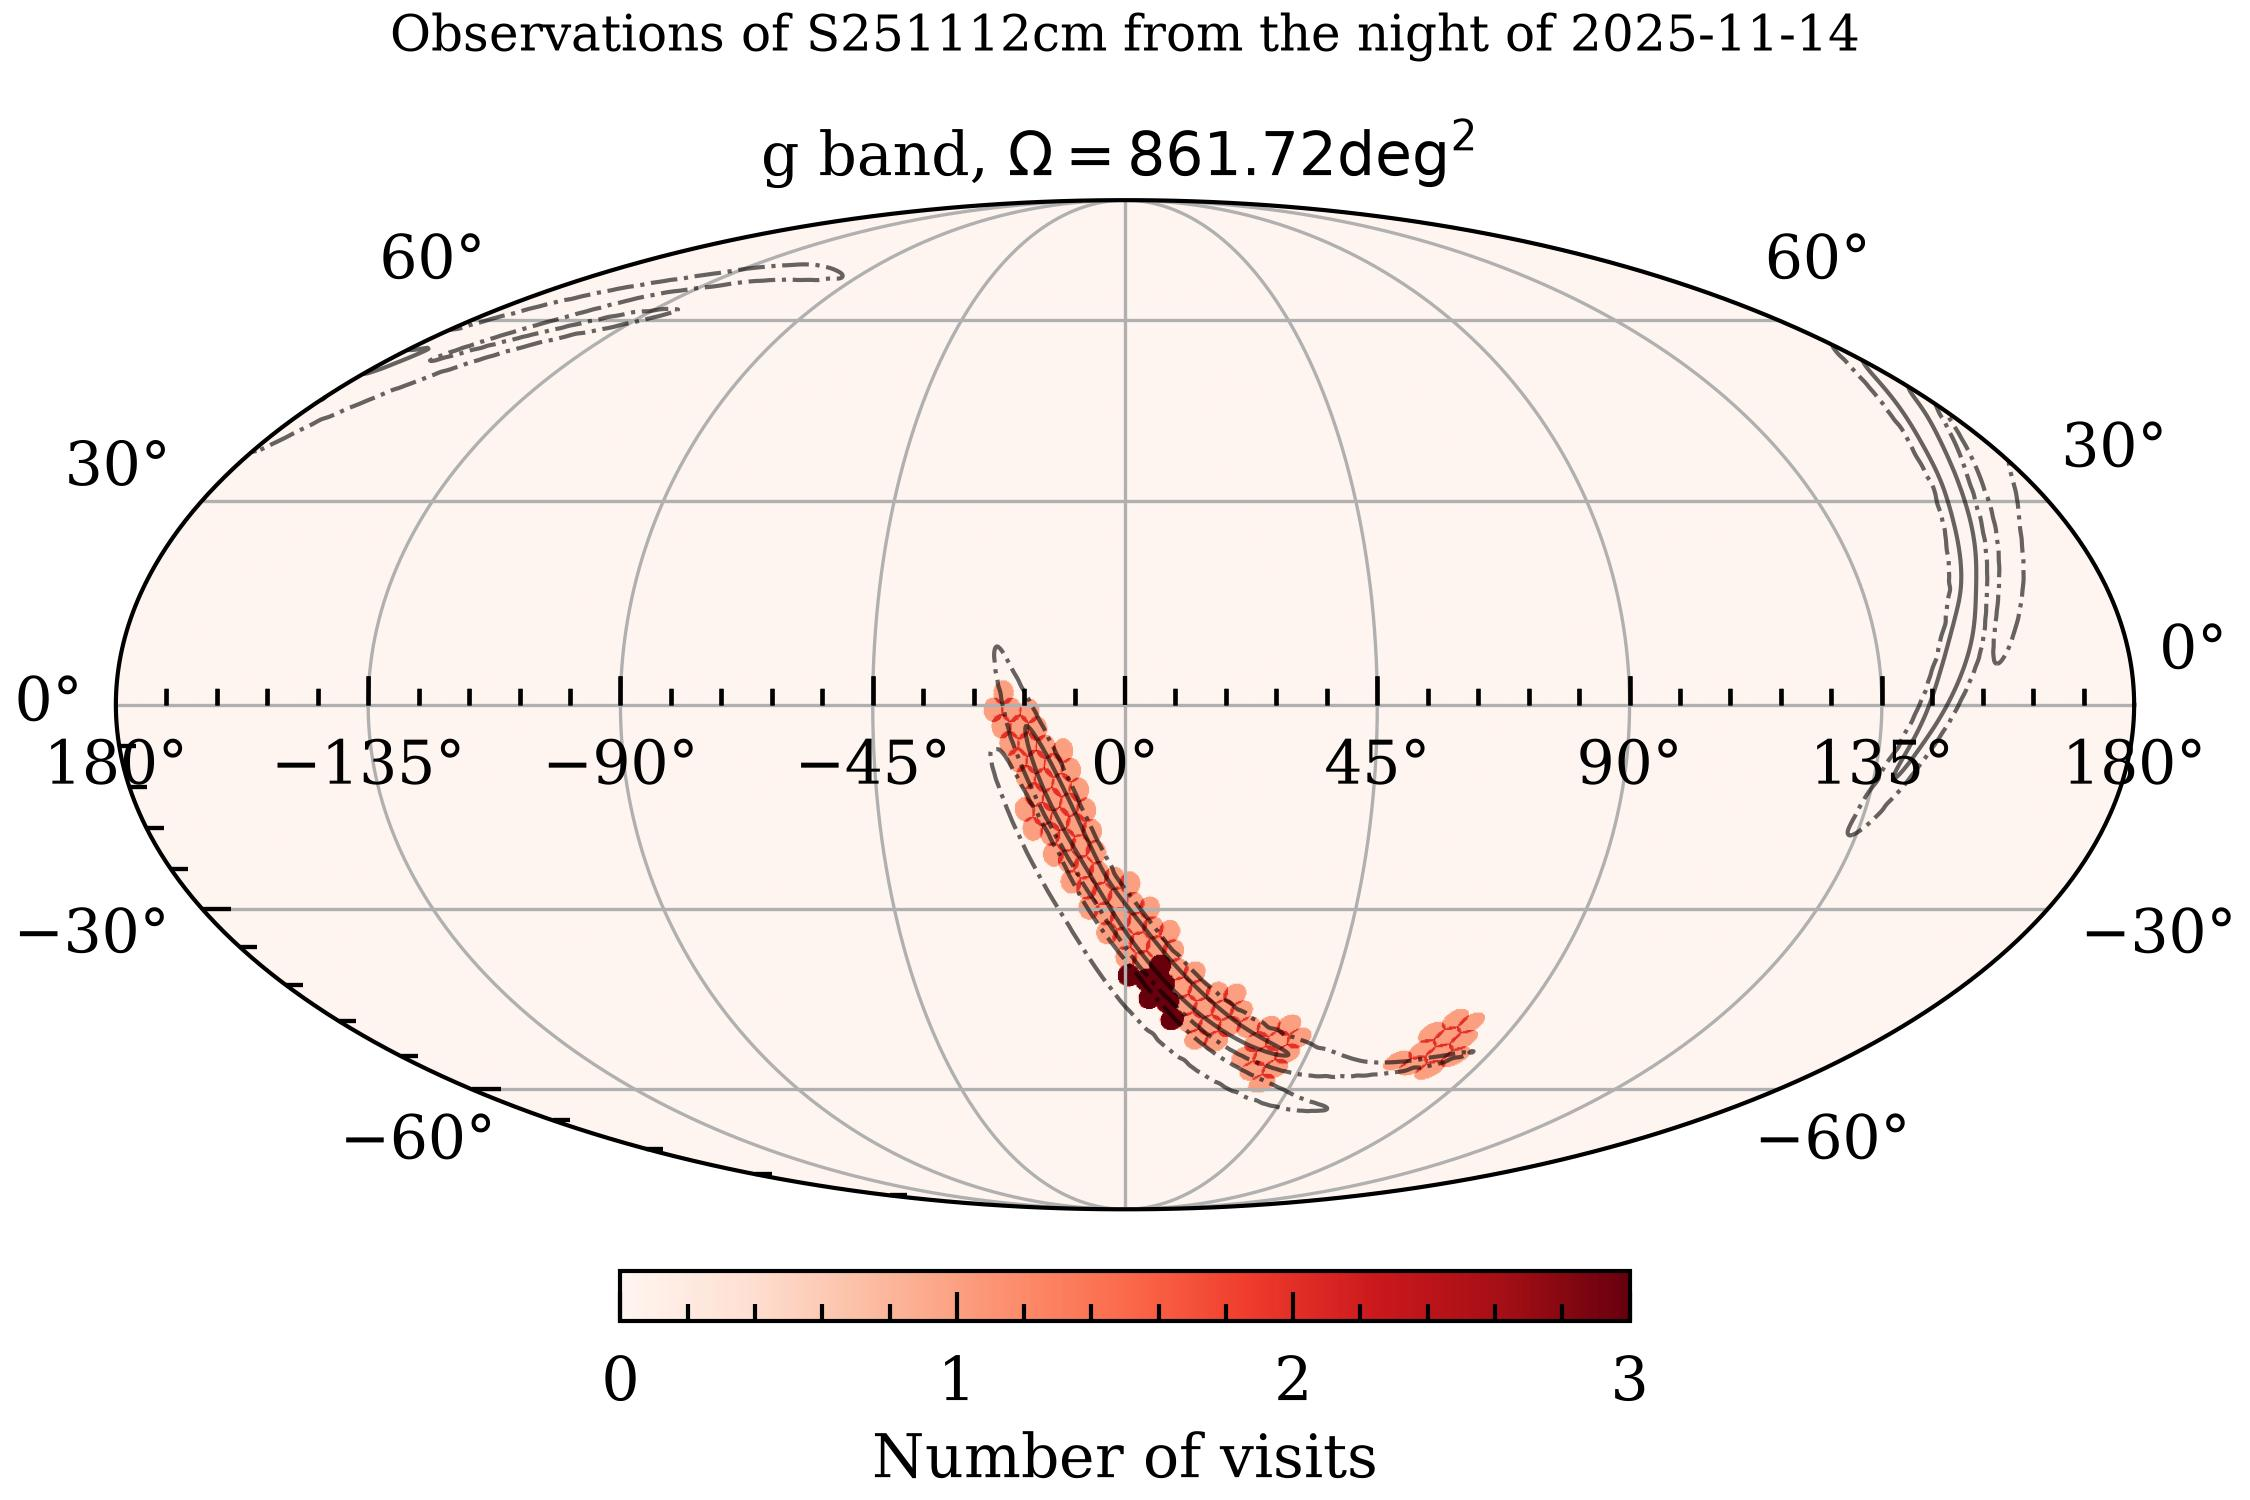
\includegraphics[width=\textwidth]{figures/20251114_obs.jpg}
        \caption{The deepest wide area ToO search to date, for GW candidate S251112cm \cite{MacBride2026RubinToO}.}
        \label{fig:highlights:s251112cm_search}
    \end{subfigure}%
    \hfill
    \begin{subfigure}[b]{0.32\textwidth}
        \centering
        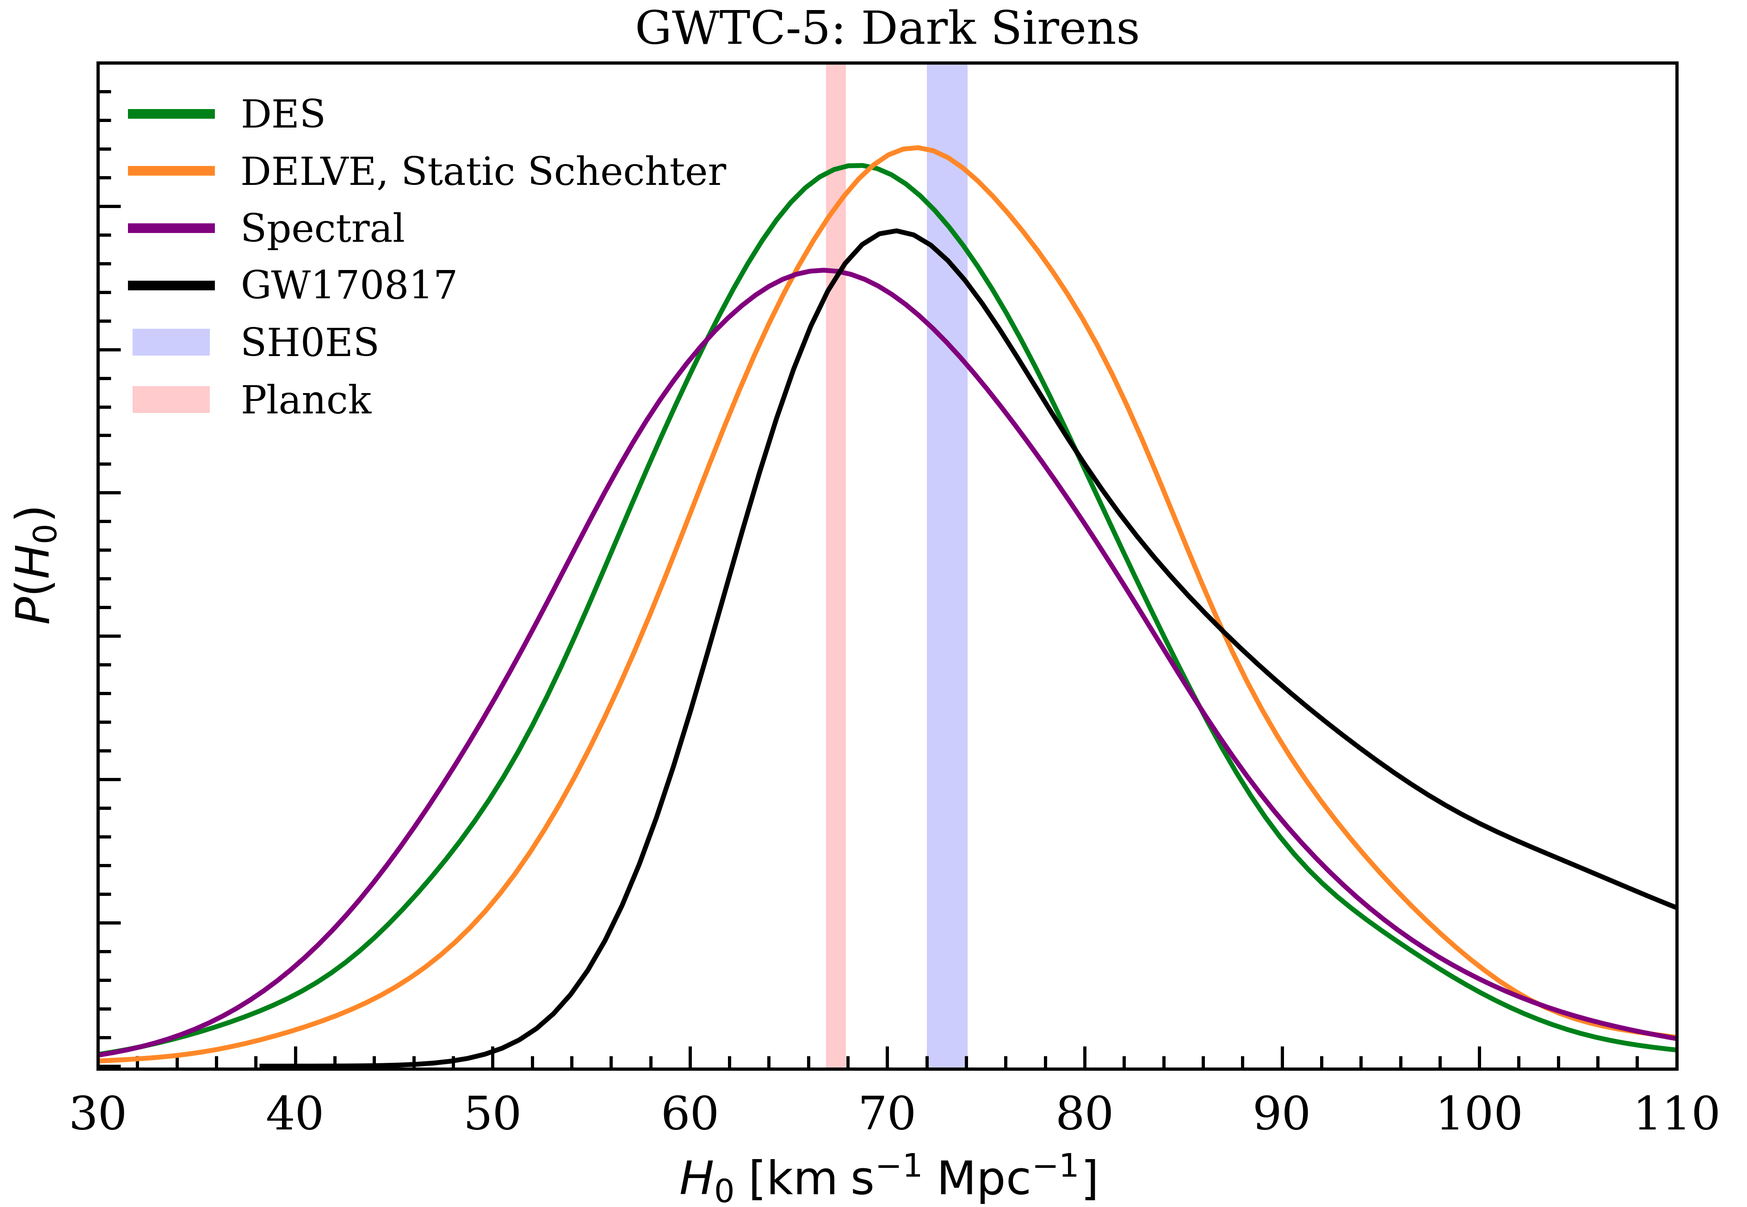
\includegraphics[width=\textwidth]{figures/delve_result.png}
        \caption{$H_0$ constraints using Gravitational Wave Transient Catalogue 5 and the DELVE galaxy catalog \cite{MacBride2026DELVEH0}.}
        \label{fig:highlights:delve_result}
    \end{subfigure}
    \caption{A summary of early career contributions, spanning instrumentation, multi-messenger astrophysics, and standard siren cosmology.}
    \label{fig:highlights}
\end{figure*}

\statement{Early Career Achievements}
My past work has been in direct support of the three pillars of my research program, and includes commissioning the focal plane array of \LSSTCam, producing the first science result for the \PFS, conducting the first \ToO\ searches for electromagnetic counterparts to gravitational waves using \Rubin, and measuring \Ho\ using the \DELVE\ galaxy catalog.

% References Figure~\ref{fig:highlights:lsstcam}, defined in the summary figure near the top of researchStatement.tex.
\textbf{Astronomical Instrumentation Development:}
My instrumentation work has encompassed both photometric and spectroscopic instruments, with a specific focus on focal plane technology.
This began with \LLAMAS, an integral field spectrograph for the Magellan Baade telescope. I validated the optical performance of the diffraction gratings and collimators for the \LLAMAS\ spectrographs, assembled and verified optical tolerance for the 24 spectrograph cameras, and integrated all 2,400 AR-coated fibers into the focal plane with zero fiber loss, before it was commissioned in 2024 \cite{Simcoe2022LLAMAS,llamas}. After integrating and testing \LLAMAS, I shifted my focus from integral-field spectrographs to multi-object spectrographs. While at the University of Michigan-Ann Arbor, I characterized and resolved a common failure mode on \DESI\ robotic positioners, known as the linear phi failure mode. While testing the \DESI\ positioners, I found that reorienting the robotic positioner to an inverted physical configuration could remove the linear phi behavior, indicating that gravity-sag has a significant influence on the failure mode \citep{Wuthrich2026Positioners}. % LLAMAS and DESI testing
% Recently, I have been testing robotic fiber positioners for next-generation spectroscopic focal planes, including the \must\ and the proposed \specsfive, and am currently leading fiber tilt-sensitivity tests of prototype positioners, including both static and dynamic measurements on a kinematic telescope mount. % Robotic positioners
This expertise with spectroscopic instruments translated effectively to the transcendent photometric imager of the next decade, the \LSSTCam. Since 2024, I have served as an \LSSTCam\ Summit Support Scientist, leading \LSSTCam\ focal-plane commissioning on Cerro Pach\'on as a key component of the in-kind contribution from Switzerland to the Rubin Project. I tested the CCDs in both the summit clean-room and on the Simonyi Survey Telescope, optimizing the sensor performance, and played a leading role in achieving \LSSTCam\ first photon in April 2024 (see Figure~\ref{fig:highlights:lsstcam}). The work to commission \LSSTCam, among other CCD optimizations, is detailed in the invited proceedings of SPIE Astronomical Telescopes + Instrumentation 2026, the most impactful astronomical instrumentation conference, held biennially \citep{MacBride2026LSSTCam}. % LSSTCam testing
% Additionally, I characterized CCD defects in the \LSSTCam\ focal plane, and developed a custom image-processing tool to monitor stability of defects during \LSSTCam operation. % LSSTCam


% References Figure~\ref{fig:highlights:s251112cm_search}, defined in the summary figure near the top of researchStatement.tex.
\textbf{Target-of-Opportunity Searches:}
I have led twenty distinct observing campaigns using different telescopes and facilities, with the goal of detecting \EM\ counterparts to \GW\ merger events. 
A variety of multi-messenger analyses are enabled by the detection of an \EM\ counterpart to a \GW\ merger event. The \textit{bright siren} method is my particular focus, which uses the redshift information of the host galaxy of an \EM\ counterpart and the luminosity distance inferred from the \GW\ source to constrain cosmology \cite{2017Natur.551...85A}.
Bright siren searches have been my primary focus while I have have been co-leading the \DESGW\ program since 2023, conducting \DECam\ observations, processing raw image data from sixteen \ToO\ campaigns to calibrated products, and analyzing processed data in response to \IGWN\ Observing Run 4 (O4) triggers.
I led a collaboration between \DESGW\ and the \JGEM\ during the O4 observing run when a well-localized gravitational wave merger candidate was accessible to both Northern and Southern hemisphere instruments. In this collaboration, I obtained multi-epoch photometry using \DECam, processed the obtained data, and cross-matched this data with spectroscopic observations using \PFS, a recently commissioned multi-object spectrograph at Subaru Telescope. This analysis enabled the first public scientific result using \PFS\ \citep{Zhang2025S250328ae}.
% This data serves a dual purpose, providing valuable transient characterization information, and also serving as the foundation for a measurement of \Ho\ using the dark siren method with spectroscopic data (see Figure~\ref{fig:pfs_coverage}).
% In addition to maintaining the day-to-day operations of the DESGW program during the IGWN O4 observing run, I improved the gravitational-wave alert-processing pipeline to provide high quality, low-latency information, to inform \ToO\ triggering decisions. Alongside improvements to the alert-processing pipeline, I augmented DESGW observing strategy by implementing changes to re-weight specific sky areas based on a variety of environmental and astrophysical conditions \TODO{Cite the MI paper, even if in-prep, plus a concrete metric from the paper}.
Since 2025, I have been leading the \Rubin\ \ToO\ observing program as the \Rubin\ \ToO\ observer. In this role, I have led observing responses to one interstellar object \citep{Chandler_2026}, one high-energy neutrino event (later reclassified as terrestrial), and two gravitational-wave merger candidates, including the deepest, wide-area \GW\ \ToO\ search to date ($m_{g,5\sigma}\sim24.8$ across $\sim850\deg^2$, see Figure~\ref{fig:highlights:s251112cm_search}) \citep{MacBride2026RubinToO,Andreoni2024RubinToO}. % Rubin ToO
% The process to build, test, and deploy an automated \ToO\ system for \Rubin\ is reflected in the recent proceedings of SPIE Astronomical Telescopes + Instrumentation 2026 \citep{MacBride2026RubinToO}, closely following the community-defined science case for the program \citep{Andreoni2024RubinToO}.

% In addition to building the \Rubin\ \ToO\ system, I have led extensive testing of the \Rubin\ \ToO\ infrastructure with the \IGWN\ and \IceCube\ collaborations, including two mock-data-challenges to assess the average latency of a \Rubin\ \ToO\ response, the accuracy of our alert processing pipeline, and the sensitivity of simulated \Rubin\ observations to optical counterparts \citep{MacBride2025MDC}\TODO{Add a metric from the mock-data-challenge}.


% References Figure~\ref{fig:highlights:delve_result}, defined in the summary figure near the top of researchStatement.tex.
\textbf{Standard Siren Constraints on the Hubble Constant:}
While recent observing campaigns have not yielded an electromagnetic counterpart to a gravitational wave merger, I have retained a focus on constraining cosmology using electromagnetic and gravitational wave data, employing the \textit{dark siren} method to measure the expansion rate of the local universe, \Ho. This work began by supporting the preparation of \DES\ data, resulting in the first dark siren constraint using a deep photometric catalog to jointly infer gravitational wave population parameters and cosmological parameters \citep{McMahon2026DESY6H0}. \DES\ was accepted as the fiducial result for the most recent \IGWN\ analysis, and demonstrated a 22\% improvement in constraining \Ho\ compared to previous analyses \citep{LVK2026GWTC5}. Building on the \DES\ analysis, I am now leading a dark-siren analysis using the \DELVE\ galaxy catalog, where initial results show \DELVE\ is competitive with \DES, obtaining a 12\% constraint on \Ho\ when combined with the bright siren GW170817 (see Figure~\ref{fig:highlights:delve_result}) \citep{MacBride2026DELVEH0}. % DES+DELVE



\statement{Future Research Activities} 
At \Institute, I will build directly on my current work in instrumentation, multi-messenger astrophysics, and standard siren cosmology to 
develop instruments for next-generation astronomical surveys,
maximize the data from \Rubin\ Observatory for bright siren measurements,
transform \LSST\ into the standard dark siren galaxy catalog,
and lead new observational programs for standard siren cosmology.

% Defines Figure~\ref{fig:pfs_coverage}, which contributions/future_new_programs.tex also references via \ref.
% If you drop this file, either keep future_new_programs.tex's figure reference intact by moving this
% wrapfigure elsewhere, or remove that reference so it doesn't render as "??".
\textbf{Astronomical Instruments to Maximize LSST data:}
In the \LSST\ era, the central bottleneck will not be imaging depth, but rather spectroscopic capacity.
% : both dark and bright siren measurements ultimately require secure redshifts of host galaxies and rapid characterization of transients from \LSST's alert stream. 
To aid in this effort, I will test and deploy advanced focal plane technology for future multi-object spectrographs.
As part of this focus, I will explore instrument design for a multi-object spectrograph optimized for standard siren cosmology, specialized for the precision and 
event rates of forthcoming gravitational wave detectors. 
This instrument would serve two goals: 1) characterize astrophysical transients associated with potential bright standard sirens, and 2) obtain spectroscopic redshifts from host galaxies to bolster dark siren measurements. Through this dual purpose, the proposed instrument would become a dark energy science machine primed to capitalize on the deluge of data from \LSST\ and future GW observatories. % MOS instrumentation development
These pathfinding activities would help to inform the proposed \specsfive, a future, large-scale cosmic frontier experiment \cite{2025arXiv250307923B}. Developing and testing of focal-plane technology will help shape the capabilities of \specsfive, so it serves as an effective spectroscopic complement to \Rubin\ starting in the mid-2030's. % Spec-S5 instrumentation development.
\begin{wrapfigure}{r}{0.5\textwidth} % 'r' for right, 'l' for left
    \centering
    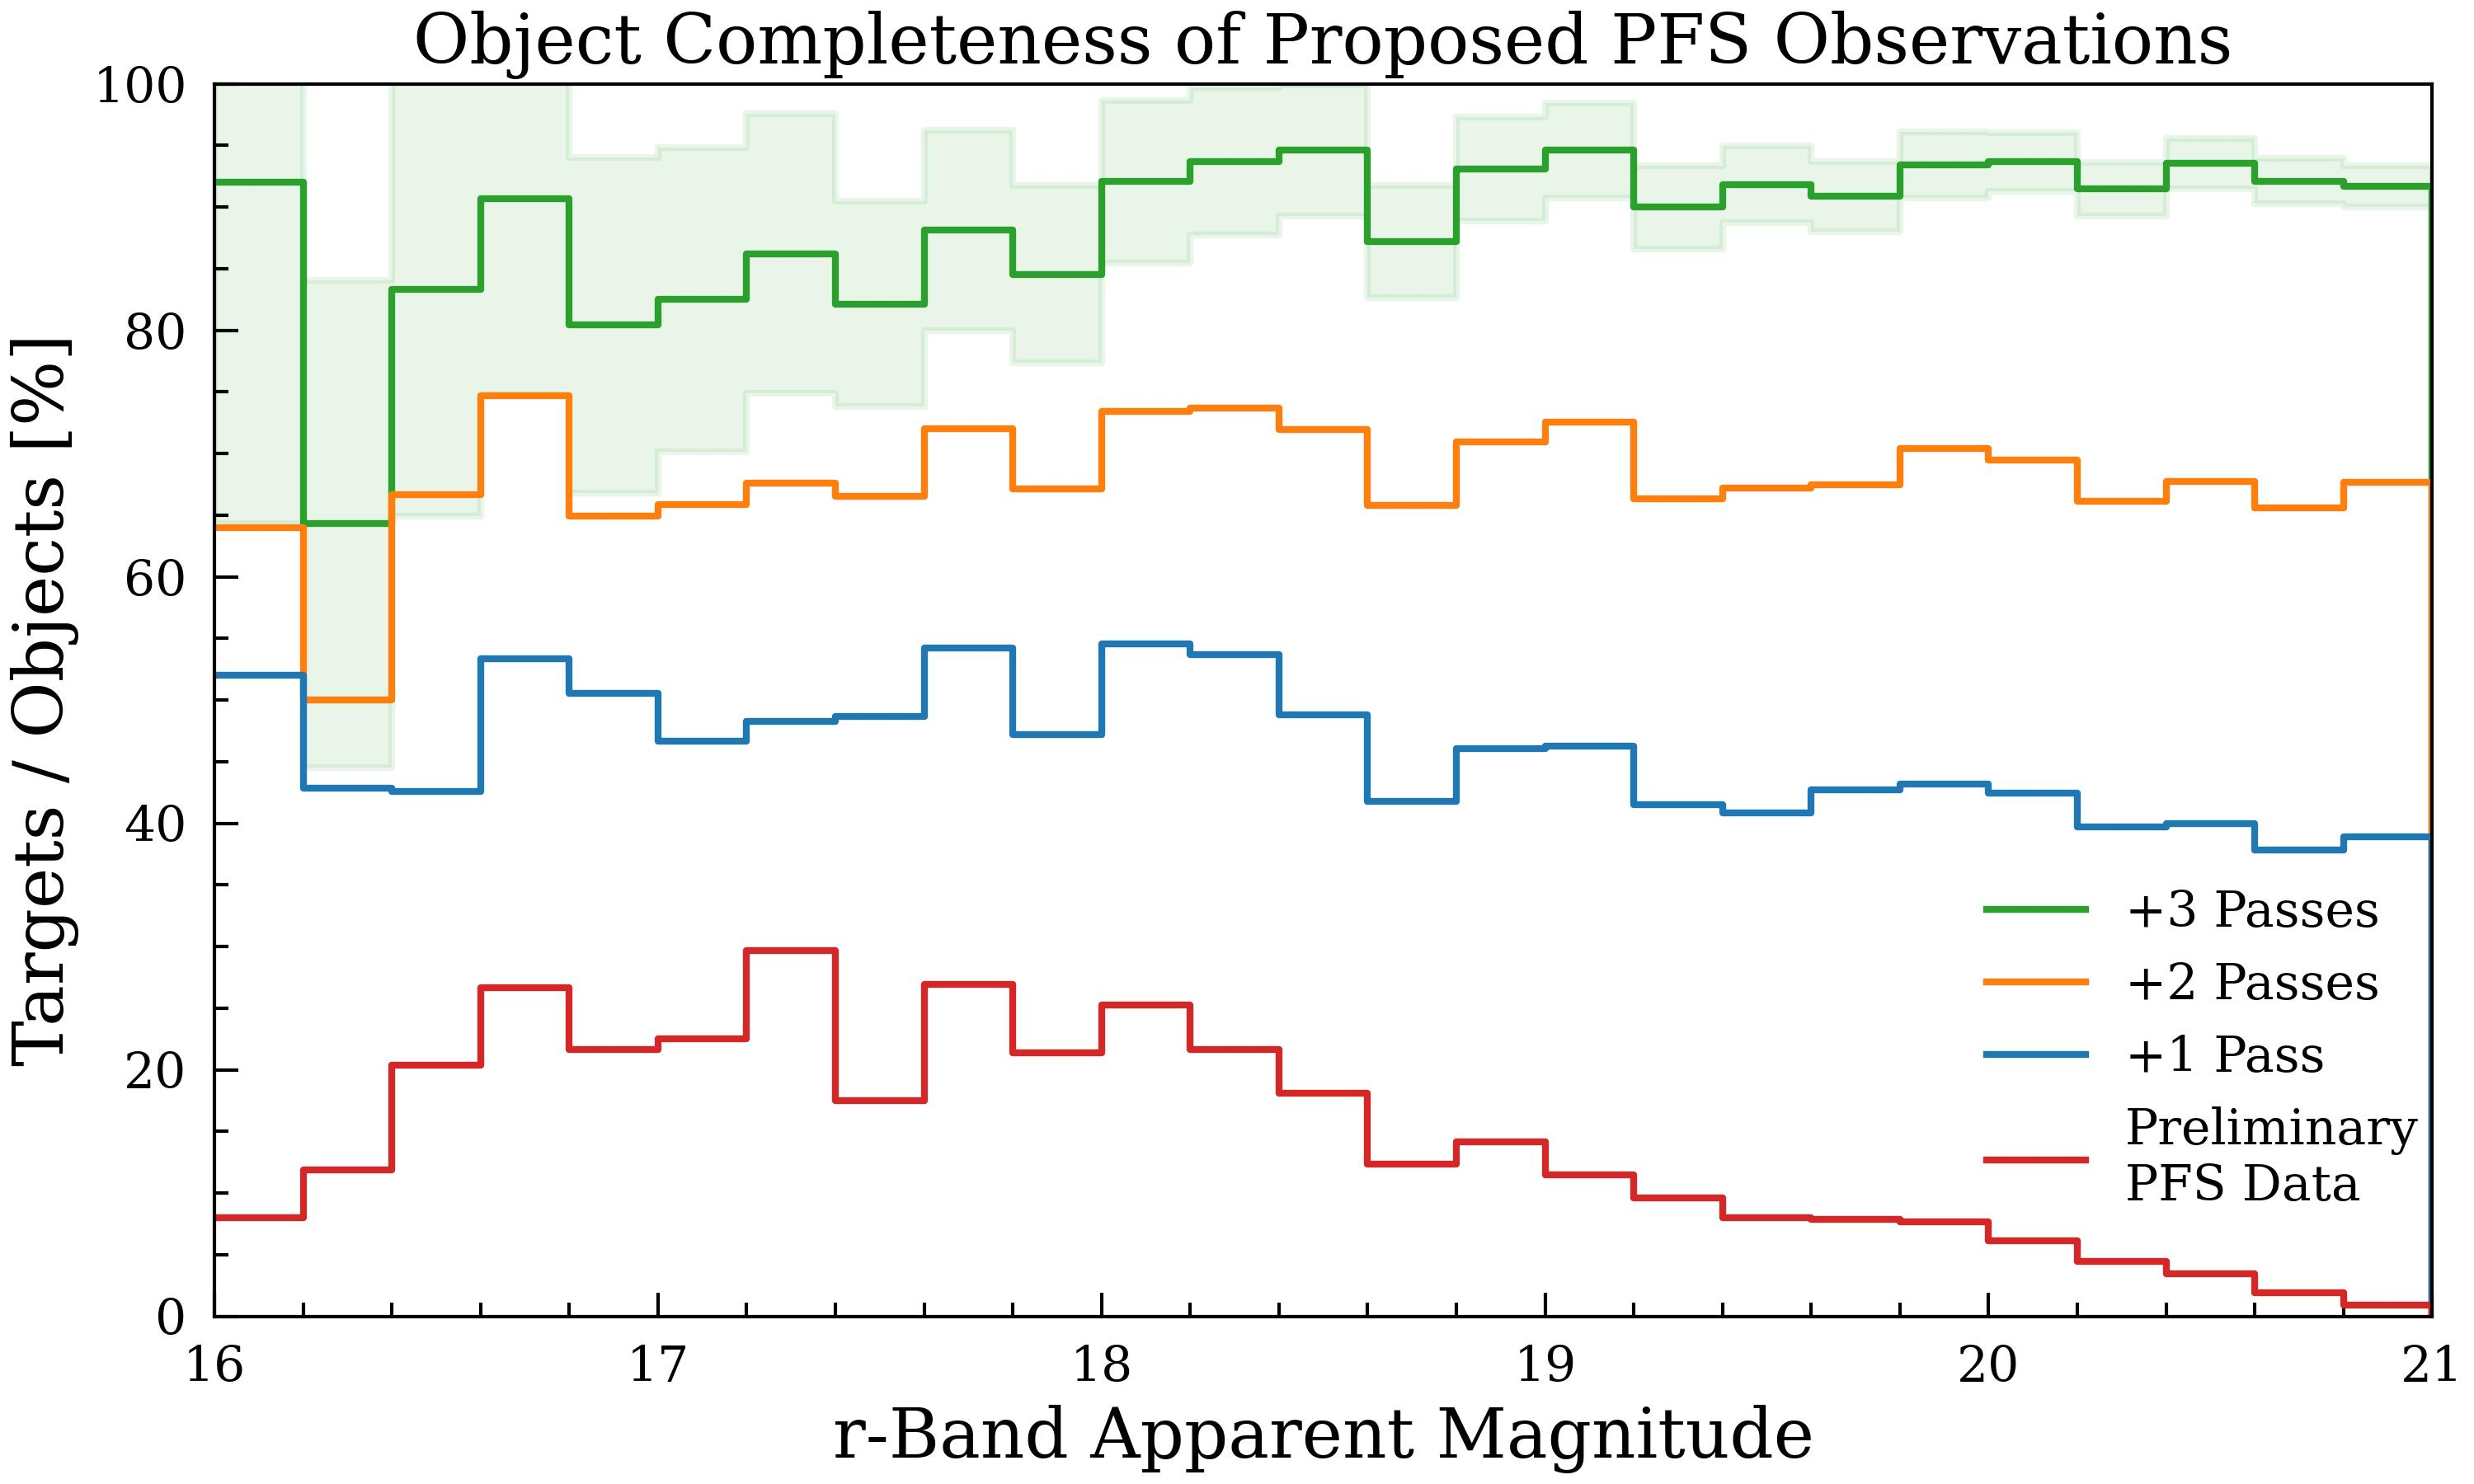
\includegraphics[width=0.5\textwidth]{figures/pfs_completeness.png}
	\caption{In red, the completeness of \PFS\ objects acquired as part of our \ToO\ campaign \cite{Zhang2025S250328ae}, with other colors showing the forecasted completeness of proposed observations. The high completeness obtained over the localization region in 3 passes (one night) demonstrates the utility of current and future multi-object spectrographs as characterization machines for standard siren cosmology.}
    \label{fig:pfs_coverage}
\end{wrapfigure}
I will continue in a support-scientist role for LSSTCam as the \LSST\ transitions into survey operations, maintaining the operational knowledge needed to respond quickly to sensor anomalies and focal-plane issues as they arise.
Building on my commissioning-era characterization of focal-plane defects, I will deploy a defect-monitoring tool, currently in-development, to \texttt{cp\_verify}, the calibration-product verification framework used by the \LSST\ Science Pipelines \cite{10.71929/rubin/2570545}. This tool will elevate defect monitoring to an automated process, directly improving the quality of \LSST\ data.

\textbf{Bright Siren Searches Enabled by Rubin Observatory:}
% Rubin ToO - drafted
I will lead the observing planning, execution, and analysis of the next bright standard siren accessible to \Rubin, along with other \ToO's pursued during the \LSST, continuing my role as the \Rubin\ \ToO\ observer throughout the transition to operations.
% This leadership is enabled by my specialized expertise in the alert processing of the \ToO\ system, my intimate knowledge of the technical strengths and limitations of the observatory, and my sustained development of the \ToO\ system within the wider \Rubin\ ecosystem.
While it is difficult to predict the timing of the next bright siren, I will continue to develop and deploy improvements to the \ToO\ system to improve response latency, observing strategy, and system automation to maximize the forthcoming opportunity to detect and characterize these optical counterparts to obtain a well-constrained measure of \Ho.
% Lead DESGW IRX analyses - observation planning, image processing, and transient analysis - drafted

In parallel to operating the \Rubin\ \ToO\ system, I will support the analysis of \DESGW\ candidates identified during \LVK\ O4, and lead the analysis of \DESGW\ candidates identified during \LVK\ intermediate runs. This work positions me to sustain and support \Rubin's \ToO\ program with additional imaging in other filters or to extended time-frames using a similarly capable photometric imager. This increased temporal sampling and color characterization will play an important role, especially as other priorities of the \LSST\ are balanced against the \ToO\ program.
% Other observing programs with spectroscopy to compliment the Rubin alert stream - in progress
As \LSST's \ToO\ program matures, I will work to enhance counterpart characterization by securing spectroscopic follow-up time on other instruments, moving beyond photometric classification to confirm spectral features that can inform the scope of \Rubin's \ToO s and constrain the physical properties of the underlying transients and their host environments. 
% This includes an ongoing program with \JGEM\ using \PFS, a new program using \LLAMAS\ to characterize promising candidates from the \LSST\ alert stream, and a future program using data from the BOOMBOX spectrograph from the Via project\TODO{Double check if applying to a Carnegie institution, otherwise swap with SOAR}.

% % Simulations of O5, 3G, and LISA source identification using Rubin
% Looking further ahead, I will begin preparing \Rubin's \ToO\ infrastructure for multi-messenger astrophysics of the future, including \threeG\ ground-based gravitational-wave detectors, the space-based \GW\ detector \LISA, new classes of high-energy neutrinos from IceCube gen-2, and the forthcoming long-baseline neutrino experiments, \DUNE\ and \hyperk. This era will usher in larger event rates, more precise localizations, and new source classes (including massive black hole mergers), that demand \ToO\ strategies tailored for a new status quo. This work will focus on identifying the optimal observing strategies for \Rubin\ discovery using \texttt{rubin\_sim} simulations along with simulated light curves, updating the alert-handling infrastructure for rapid processing, and strengthening follow-up partnerships across a variety of other observatories and experiments. Enhancing the detection of counterparts associated with \GW\s from \threeG\ and space-based detectors will extend the standard siren lever arm for precision cosmology, enabling measurements of $\Omega_m$, $w$, and other dark energy models.


%% LSST efforts for dark sirens
\textbf{LSST data for Dark Siren Cosmology:}
I will pursue a cutting-edge program that produces a gold-standard galaxy catalog for dark siren cosmology using \LSST\ data.
% LSST DP2 characterization in prep for DR1
This program proceeds in four stages, each building towards a powerful, world leading measurement.
It begins with an ongoing project, focused on characterizing the \LSST\ Data Preview 2 (DP2) galaxy catalog, focusing on robust object classification that is scalable to future \LSST\ data releases.\TODO{Could reference Andres paper if it is published soon-ish}
% DESC Y1 forecasting
Following characterization of DP2, I will finish a forecasting study that quantifies the $H_0$ precision achievable by combining simulated first-year LSST data with an O4-like gravitational-wave catalog, extending the dark-siren methodology from my recent \DELVE\ measurement to project the constraining power in the \LSST\ era.
% LSST DR1 measurement
Superceding DP2 characterization and forecasted precision, I will characterize the first LSST Data Release (DR1) galaxy catalog and produce a dark siren measurement of $H_0$. This result will extend the methodology I developed with \DELVE\ to a dataset with substantially greater depth, area, and photometric uniformity, all features that will make it the standard galaxy catalog for dark siren analyses.
% LSST DR1 combined probes - emphasize shear instead of clustering
Building on the DR1 measurement, I aim to combine \LSST\ large-scale structure measurements in a joint cosmological analysis, using cosmic shear and standard sirens to obtain a tighter constraint of $H_0$, and extend the constraints to $\Omega_m$.


% References Figure~\ref{fig:pfs_coverage}, defined in contributions/future_instrumentation.tex.
% If that file is dropped, this reference will render as "??" unless you remove or update it.
\textbf{New Observational Programs and Analyses for Standard Sirens:}


\begin{wrapfigure}{lb}{0.45\textwidth} % 'r' for right, 'l' for left
    \centering
    \includegraphics[width=0.42\textwidth]{figures/placeholder.pdf}
    \caption{Caption for wrapped image.}
    \label{fig:future_work}
\end{wrapfigure}

These plans form one continuous arc, not separate agendas. The near-term focus on builds the operational standing and analysis pipelines within \Rubin, \LSST, and \LVK, and provides the basis for executing on the longer-term program. 
That foundation will enable impactiful standard-siren measurements, a pioneering specialized survey for gravitational wave cosmology, combined-probe analyses in LSST-DESC, and instrumentation development to maximize the 2030's using both spectroscopic and photometric instruments.
\bigskip
\statement{References}
{\small A full publication list is available on \href{https://scholar.google.com/citations?user=XtRTswUAAAAJ}{Google Scholar} and \href{https://ui.adsabs.harvard.edu/search/q=((author%3A%22MacBride%2C%20S.%22)%20AND%20year%3A2017-2100)&sort=date%20desc%2C%20bibcode%20desc&ui_tag=results%2Fgraph%2Fyear&p_=0}{NASA ADS} (h-index \hindex\ as of \hindexDate).}
\renewcommand{\refname}{}
\vspace{-2\baselineskip}
{\small\bibliography{references}}

\end{document}
